
%(BEGIN_QUESTION)
% Copyright 2006, Tony R. Kuphaldt, released under the Creative Commons Attribution License (v 1.0)
% This means you may do almost anything with this work of mine, so long as you give me proper credit

Complete the following ladder-logic schematic diagram for part of a steam boiler control system, inserting the correct types of pressure switches in the correct locations, complete with all necessary interconnecting wires:

$$\includegraphics[width=15.5cm]{i00465x01.eps}$$

One pressure switch, set at 185 PSI, controls the high steam pressure warning lamp, energizing the lamp if the steam pressure ever exceeds 185 PSI.  Another pressure switch, set at 110 PSI, controls the secondary burner fuel solenoid, firing this burner if the steam pressure ever falls below 110 PSI.  The final pressure switch is set at 205 PSI, and is used to completely shut down the boiler by shutting (``tripping'') the fuel trip solenoid valve if the steam pressure ever exceeds this setting.

\vskip 10pt

\noindent
Credit will be given for correctly wiring each of the three branch circuits.  You {\it must} write the given pressure setting (in PSI) next to each switch in order to receive credit for that circuit:

\begin{itemize}
\item{} High steam pressure warning lamp
\item{} Secondary burner fuel solenoid
\item{} Fuel trip solenoid valve
\end{itemize}

\underbar{file i00465}
%(END_QUESTION)





%(BEGIN_ANSWER)

$$\includegraphics[width=15.5cm]{i00465x02.eps}$$

3 points for warning lamp and solenoid valve switches each, 4 points for secondary burner switch.

%(END_ANSWER)





%(BEGIN_NOTES)

{\bf This question is intended for exams only and not worksheets!}.

%(END_NOTES)


